%\subsubsection{Tiny Code Generator}
%\label{chap:qemu_tcg}

QEMU's DBT takes the named of the Tiny Code Generator (TCG), and the basic 
code fragments it analyzes are called Translation Blocks (TB). In the case of QEMU's 
TCG, the TBs are defined by using any instruction that changes the control flow of 
the program—jump or return instructions, interruptions or peripherals accesses—as 
boundaries\cite{QemuTCGOpsDevel}\cite{QemuTCGDirectBlockChaining}.

The translation performed by the TCG consists of two phases: converting the host 
code into a sequence of micro-operations and turning these micro-operations 
into executable code\cite{QemuTCGTechReport}. The figure \ref{fig:tcg} illustrates the general architecture and 
workflow of the TCG. Where the "Destination Machine Code" corresponds to a TB, the 
XXX portion of the diagram represents the TCG, and the last block represents the 
"Host Machine Code".

\begin{figure}[H]
    \centering
%    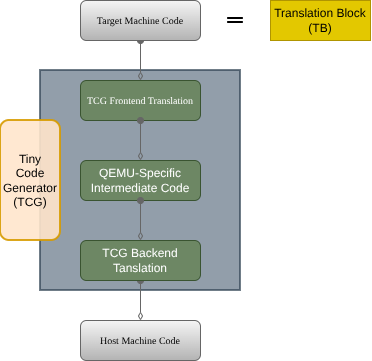
\includegraphics[width=0.5\textwidth]{Resources/Draw/TCG.png}
    \caption{Tiny Code Generator}
    \label{fig:tcg}
\end{figure}

In the first phase, the TCG's frontend section decomposed each guest instruction 
from the corresponding TB into equivalent sequences of QEMU-specific intermediate 
representations (IRs), called micro-operations. Conceptually, these micro-operations 
are like an assembly language designed specifically for QEMU's compilation infrastructure.

In the second phase, the TCG's back-end section converts this intermediate 
representation into native host machine code, which is then directly executable on 
the host processor\cite{QemuTCGFrontendOps}\cite{QemuTCGBackendOps}. The TCG maintains a dictionary of micro-operations. 
This dictionary contains a mapping between micro-operations and the equivalent 
sequences of host architecture binary code. This binary code performs the task of 
the corresponding micro-operation when run on the host processor. The TCG cycles 
through each micro-operation contained in the translation block and emits the 
corresponding sequence of host machine instructions by using the dictionary. 
The result is a block of host machine code that performs the same operations as the 
guest machine code\cite{QemuTCGTechReport}.

The QEMU developers' decision to separate front-end and back-end translation 
was a wise one, as it offers significant advantages for QEMU's scalability. Thanks 
to this decision, to support a new host CPU architecture, developers only need to 
implement a new front-end translator, while the back-end translation logic remains 
unchanged. Conversely, supporting QEMU on a new host architecture only requires 
back-end development, without affecting compatibility with that architecture. This 
modularity is the primary reason for QEMU's scalability across various hardware 
platforms and CPU architectures.

